\documentclass[11pt]{article}
\usepackage{array}
\usepackage{tabularx}
\usepackage{graphicx}
\usepackage{listings}
\title{
	\textbf{Autonomous Agents Assignment 1}
}

\author{Tobias Stahl \\ 10528199 \and Spyros Michaelides \\ 10523316 \and Ioannis Giounous Aivalis \\ 10524851 \and Francesco Stablum \\ 6200982}
\usepackage{graphicx}
\begin{document}

\maketitle

\section{Introduction}
This report will discuss the predator vs. prey world Markov Decision Process (MDP). The environment is is a toroidal grid in which, if an agent moves off the boundary of the side of the grid, he will appear at the opposite side of the board. The board has a size of 11 by 11 cells.\\
Both the predator and the prey move with a random policy inclusive of directions NORTH, SOUTH, WEST, EAST along with an option of staying still. While the predator has a 0.2 probability of taking any action, the prey has a probability 0.8 of staying in the same cell, and moves with a probability of only 0.05 in any direction.\\
The probability for an action taken by the prey is changed when the predator will be standing next to it, as the prey is not allowed to move into the predator. This will change the probability of the prey moving to 0.067 toward any of the remaining directions.\\
The goal of the predator is to catch the prey which occurs when the predator moves into the prey. The reward for catching the prey is 10 and the immediate reward for any other action is 0.\\
The entire MDP is known to the agent, which means that the agent (predator) can determine the optimal policy before interacting with the environment.


\section{Methods}
The following part explains the methods that are used to complete the assignment which is described in this report.


\subsection{State Representation}
The given state representation is one where the state is represented by two pairs of coordinates, where one pair corresponds to the location of the predator and the other to the one of the prey. There are four possible states for each given coordinate, therefore the state space complexity is bound to $O(n^4)$.
The possible states for each (x,y) coordinate are the following:
\begin{itemize}
	\item Both actors are placed on the given coordinate.
	\item None of the actors stand on the given coordinate.
	\item Only the prey is located on the given coordinate.
	\item Only the predator is situated on the given coordinate.
\end{itemize}
Given that the size of the board is 11, the size of the state space is equal to $11 \times 11 \times 11 \times 11$.


\subsection{Reduced State Representation}
For the reduced state space, the assumption was made that only the prey moves and the predator is considered static, i.e. it stays in a fixed position. Because of the grid being toroidal and the equivalence of the states that represent the same relative position between the predator and the prey, the state space can be reduced from O($n^4$) to O($n^2$). Whenever the predator moves, only the prey is considered to move into the opposite direction.\\
For example, given that the prey is located in (5,5), the predator in (0,0); given that the predator takes action SOUTH, the resulting state would be equivalent to one in which the predator stays in (0,0) and the prey moves NORTH to (4,5).



\subsection{Simulator}
In the simulator the prey and predator move according to their policy until the prey is caught by the predator. The coordinates of both the agent and the prey are initialized in the beginning of each episode.


\subsection{Iterative Policy Evaluation}
An iterative policy evaluation is used to determine the value for all possible states, using a discount factor of 0.8.\\
The value of a state is determined by summing the expected reward and value of all possible next states s' multiplied by the probability of actually moving into this state s'.\\
This is repeated as long as the policy keeps changing. Once this stops, the best policy is found.\\
The policy evaluation will stop once the change in values is smaller than threshold Theta, where Theta is 0.00000001.\\\\


\subsection{Policy Iteration}
Policy Iteration has been implemented in order to find an optimal policy.
Once all the states are evaluated using Policy Evaluation (explained in part 2), a policy improvement algorithm is used to find the best action for the predator to take, regarding the reward to expect in the next state.\\
In order to do this the best action for each state is chosen by changing the probability of taking this action in this state to 1.0, while the rest of the actions in the state are reduced to a probability of 0. \\
Because of this change of probabilities the states need to be re-evaluated, leading to an iterative process until the policy is stable.


\subsection{Value Iteration}
One of the disadvantages in using policy iteration is that policy evaluation might need multiple sweeps through the state space, in order to converge. The difference between value iteration and policy iteration, is that "Value iteration effectively combines, in each of its sweeps, one sweep of policy evaluation and one sweep of policy improvement." \\



\section{Results\\}


\subsection{Simulation}
In order to find the average of moves it takes the predator to catch the prey using the random policy a simulation of 100 runs is made. The resulting value for the average is 245.06 steps with a standard deviation of 205.836.\\



\subsection{Iterative Policy Evaluation}


Stated below are the values found by policy evaluation for sample states:\\\\
$\bullet$ Predator(0,0), Prey(5,5) $\Rightarrow 0.0089872$\\\\
$\bullet$ Predator(2,3), Prey(5,4) $\Rightarrow  0.2859599$\\\\
$\bullet$ Predator(2,10), Prey(10,0) $\Rightarrow  0.2859599$\\\\
$\bullet$ Predator(10,10), Prey(0,0) $\Rightarrow  1.9428952$\\\\
The algorithm took a total of 40 iterations to converge to the limit.\\

\subsection{Policy Iteration}
The output of the values of all states in which the prey is located at (5,5), using Policy Iteration with a discount factor of $\gamma$=0.8, is displayed in Table ~\ref{table:outputPolIter}.
The values for the set of discount factors are shown in the Table~\ref{table:discFactors} below. It can be seen that policy iteration takes more execution time, given the fact that policy iteration performs policy evaluation on every iteration this is to be expected.
\begin{center}
\begin{table*}[ht]
{\small
\hfill{}
\begin{tabular}{c|c|c|c|c}
 &  \textbf{Policy Iteration} &  & \textbf{Value Iteration} &\\
\textbf{Discount Factor} &  \textbf{Iterations} & \textbf{Seconds} & \textbf{Iterations} & \textbf{Seconds}\\
	\hline
0.1 & 13 & 16.4 & 7 & 3.3\\
0.5 & 15 & 44.4 & 19& 7\\
0.7 & 18 & 54 & 34& 12.3\\
0.9 & 11 & 80.9 & 110& 37.7\\
\end{tabular}}
\hfill{}
\caption{Number of iterations and execution time for different discount factors.}
\label{table:discFactors}
\end{table*}
\end{center}





\subsection{Value Iteration}
The output of the values of all states in which the prey is located at (5,5), using Value Iteration with a discount factor of $\gamma$=0.8, is displayed in Table ~\ref{table:outputValIter}.
\begin{center}
\begin{table*}[ht]
{\small
\hfill{}
\begin{tabular}{c|c|c|c|c|c|c|c|c|c|c|c}
\textbf{} & \textbf{0} & \textbf{1} & \textbf{2} & \textbf{3} & \textbf{4} & \textbf{5} & \textbf{6} & \textbf{7} & \textbf{8} & \textbf{9} & \textbf{10}\\
	\hline
\textbf{0} & 5.504 & 6.716 &
8.447 & 10.560 & 13.107 & 15.392 & 12.943 & 10.524 & 8.562 & 6.930 & 5.555\\
\textbf{1} & 6.797 & 8.447 & 10.560 & 13.107 & 16.347 & 19.515 & 16.282 & 12.943 & 10.508 & 8.461 & 6.800\\
\textbf{2} & 8.472 & 10.481 & 13.099 & 16.343 & 20.338 & 24.736 & 19.930 & 16.068 & 13.027 & 10.369 & 8.427\\
\textbf{3} & 10.481 & 13.099 & 16.343 & 20.338 & 24.736 & 31.477 & 24.736 & 19.930 & 16.068 & 13.027 & 10.369\\
\textbf{4} & 12.103 & 15.233 & 19.402 & 24.710 & 31.477 & 39.999 & 31.477 & 24.710 & 19.402 & 15.233 & 12.103\\
\textbf{5} & 15.233 & 19.402 & 24.710 & 31.477 & 39.999 & 39.999 & 39.999 & 31.477 & 24.710 & 19.402 & 15.233\\
\textbf{6} & 12.103 & 15.233 & 19.402 & 24.710 & 31.477 & 39.999 & 31.477 & 24.710 & 19.402 & 15.233 & 12.103\\
\textbf{7} & 10.486 & 13.100 & 16.343 & 20.338 & 24.736 & 31.477 & 24.736 & 19.962 & 16.277 & 12.897 & 10.348\\
\textbf{8} & 8.4767 & 10.486 & 13.100 & 16.343 & 20.338 & 24.736 & 19.962 & 16.277 & 12.897 & 10.348 & 8.447\\
\textbf{9} & 6.872 & 8.468 & 10.539 & 13.107 & 16.347 & 19.515 & 16.326 & 13.071 & 10.518 & 8.387 & 6.855\\
\textbf{10} & 5.570 & 6.798 & 8.468 & 10.539 & 13.107 & 15.404 & 13.071 & 10.518 & 8.387 & 6.783 & 5.558\\
\end{tabular}}
\hfill{}
\caption{Using Policy Iteration: Values of all states in which the prey is located at (5,5) with a discount factor of ($\gamma$=0.8), convergence after 16 iterations.}
\label{table:outputPolIter}
\end{table*}
\end{center}



\begin{center}
\begin{table*}[ht]
{\small
\hfill{}
\begin{tabular}{c|c|c|c|c|c|c|c|c|c|c|c}
\textbf{} & \textbf{0} & \textbf{1} & \textbf{2} & \textbf{3} & \textbf{4} & \textbf{5} & \textbf{6} & \textbf{7} & \textbf{8} & \textbf{9} & \textbf{10}\\
	\hline
\textbf{0} & 5,664 & 6,988 & 8,617 & 10,619 & 13,122 & 15,410 & 13,122 & 10,619 & 8,617 & 6,988 & 5,664\\
\textbf{1} & 6,988 & 8,517 & 10,591 & 13,175 & 16,365 & 19,521 & 16,365 & 13,175 & 10,591 & 8,517 & 6,988\\
\textbf{2} & 8,617 & 10,591 & 13,175 & 16,391 & 20,390 & 24,766 & 20,390 & 16,391 & 13,175 & 10,591 & 8,617\\
\textbf{3} & 10,619 & 13,175 & 16,391 & 20,390 & 25,375 & 31,477 & 25,375 & 20,390 & 16,391 & 13,175 & 10,619\\
\textbf{4} & 13,122 & 16,365 & 20,390 & 25,375 & 31,477 & 40,000 & 31,477 & 25,375 & 20,390 & 16,365 & 13,122\\
\textbf{5} & 15,410 & 19,521 & 24,766 & 31,477 & 40,000 & 40,000 & 40,000 & 31,477 & 24,766 & 19,521 & 15,410\\
\textbf{6} & 13,122 & 16,365 & 20,390 & 25,375 & 31,477 & 40,000 & 31,477 & 25,375 & 20,390 & 16,365 & 13,122\\
\textbf{7} & 10,619 & 13,175 & 16,391 & 20,390 & 25,375 & 31,477 & 25,375 & 20,390 & 16,391 & 13,175 & 10,619\\
\textbf{8} & 8,617 & 10,591 & 13,175 & 16,391 & 20,390 & 24,766 & 20,390 & 16,391 & 13,175 & 10,591 & 8,617\\
\textbf{9} & 6,988 & 8,517 & 10,591 & 13,175 & 16,365 & 19,521 & 16,365 & 13,175 & 10,591 & 8,517 & 6,988\\
\textbf{10} & 5,664 & 6,988 & 8,617 & 10,619 & 13,122 & 15,410 & 13,122 & 10,619 & 8,617 & 6,988 & 5,664\\
\end{tabular}}
\hfill{}
\caption{Using Value Iteration: Values of all states in which the prey is located at (5,5) with a discount factor of ($\gamma$=0.8), convergence after 53 iterations.}
\label{table:outputValIter}
\end{table*}
\end{center}
\pagebreak


\section{Implementation} 
\begin{figure}[!ht]
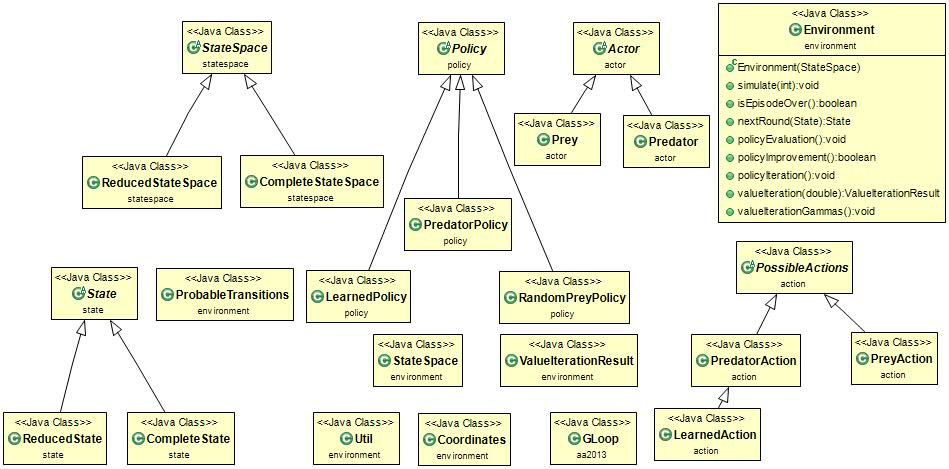
\includegraphics[scale=0.5]{pic.jpg}
\caption{The UML diagram above displays the classes used to implement the assignment exercise.}
\label{UML}
\end{figure}


\section{Conclusion}
In this assignment about Single Agent Planning in a fully observable Markov Decision Process, different algorithms were used to find an optimal policy for an agent to catch a prey. Policy evaluation is used to determine the value of states for the agent's policy. In order to improve the policy, policy iteration and value iteration have been implemented, with the awareness that policy iteration needs less iteration steps, but value iteration finds the best policy faster.


\begin{thebibliography}{3}

[Sutton and Barto, 1998] Sutton, R. S. and Barto, A. G. (1998). Reinforcement learning: An introduction.

\end{thebibliography}




\section{Appendix}

The package 'aa2013'only contains \texttt{'GLoop.java'} with the main method.

The package \texttt{'action'} contains the probabilities to take an action.\\
It contains the  following classes:

\begin{itemize}
	\item \texttt{'LearnedAction.java'}
	\item \texttt{'PossibleActions.java'}
	\item \texttt{'PredatorAction.java'}
	\item \texttt{'PreyAction.java'}
\end{itemize}

The package \texttt{'actor'} contains the classes with the constructors for prey and predator:

\begin{itemize}
	\item \texttt{'Actor.java'}
	\item \texttt{'Predator.java'}
	\item \texttt{'Prey.java'}
\end{itemize}

The package \texttt{'environment'} contains the following classes:\\
All algorithms are impemented there.

\begin{itemize}
	\item \texttt{'Coordinates.java'}
	\item \texttt{'Environment.java'}
	\item \texttt{'ProbableTransitions.java'}
	\item \texttt{'StateSpace.java'}
	\item \texttt{'Util.java'}
	\item \texttt{'ValueIterationResult.java'}
\end{itemize}

The package \texttt{'policy'} contains the classes:

\begin{itemize}
	\item \texttt{'LearnedPolicy.java'}
	\item \texttt{'Policy.java'}
	\item \texttt{'PredatorPolicy.java'}
	\item \texttt{'RandomPreyPolicy.java'}
\end{itemize}

The package \texttt{'state'} contains the classes:

\begin{itemize}
	\item \texttt{'CompleteState.java'}
	\item \texttt{'ReducedState.java'}
	\item \texttt{'State.java'}
\end{itemize}

The package \texttt{'statespace'} contains the classes:

\begin{itemize}
	\item \texttt{'CompleteStateSpace.java'}
	\item \texttt{'ReducedStateSpace.java'}
	\item \texttt{'StateSpace.java'}
\end{itemize}


The package \texttt{'state'} contains the classes:

\begin{itemize}
	\item \texttt{'LearnedAction.java'}
	\item \texttt{'PossibleActions.java'}
	\item \texttt{'PredatorAction.java'}
	\item \texttt{'RandomPreyAction.java'}
\end{itemize}

\end{document}
